% This file defines the command for the combined forward/backward pass diagram.
% It can be compiled standalone or included in a larger document.

\ifdefined\ispartofbook
\else
  % --- Standalone Compilation Preamble ---
  \documentclass[tikz, border=10pt]{standalone}
  \usepackage{amsmath, amssymb} % For math symbols
  \usepackage{tikz}
  \usetikzlibrary{
    positioning,
    arrows.meta,
    fit,
    decorations.pathreplacing,
    calligraphy,
    shapes.geometric,
    shadows,
    chains,
    backgrounds
  }
  \begin{document}
\fi

% --- THE DIAGRAM COMMAND ---
\newcommand{\combineddiagram}{%
    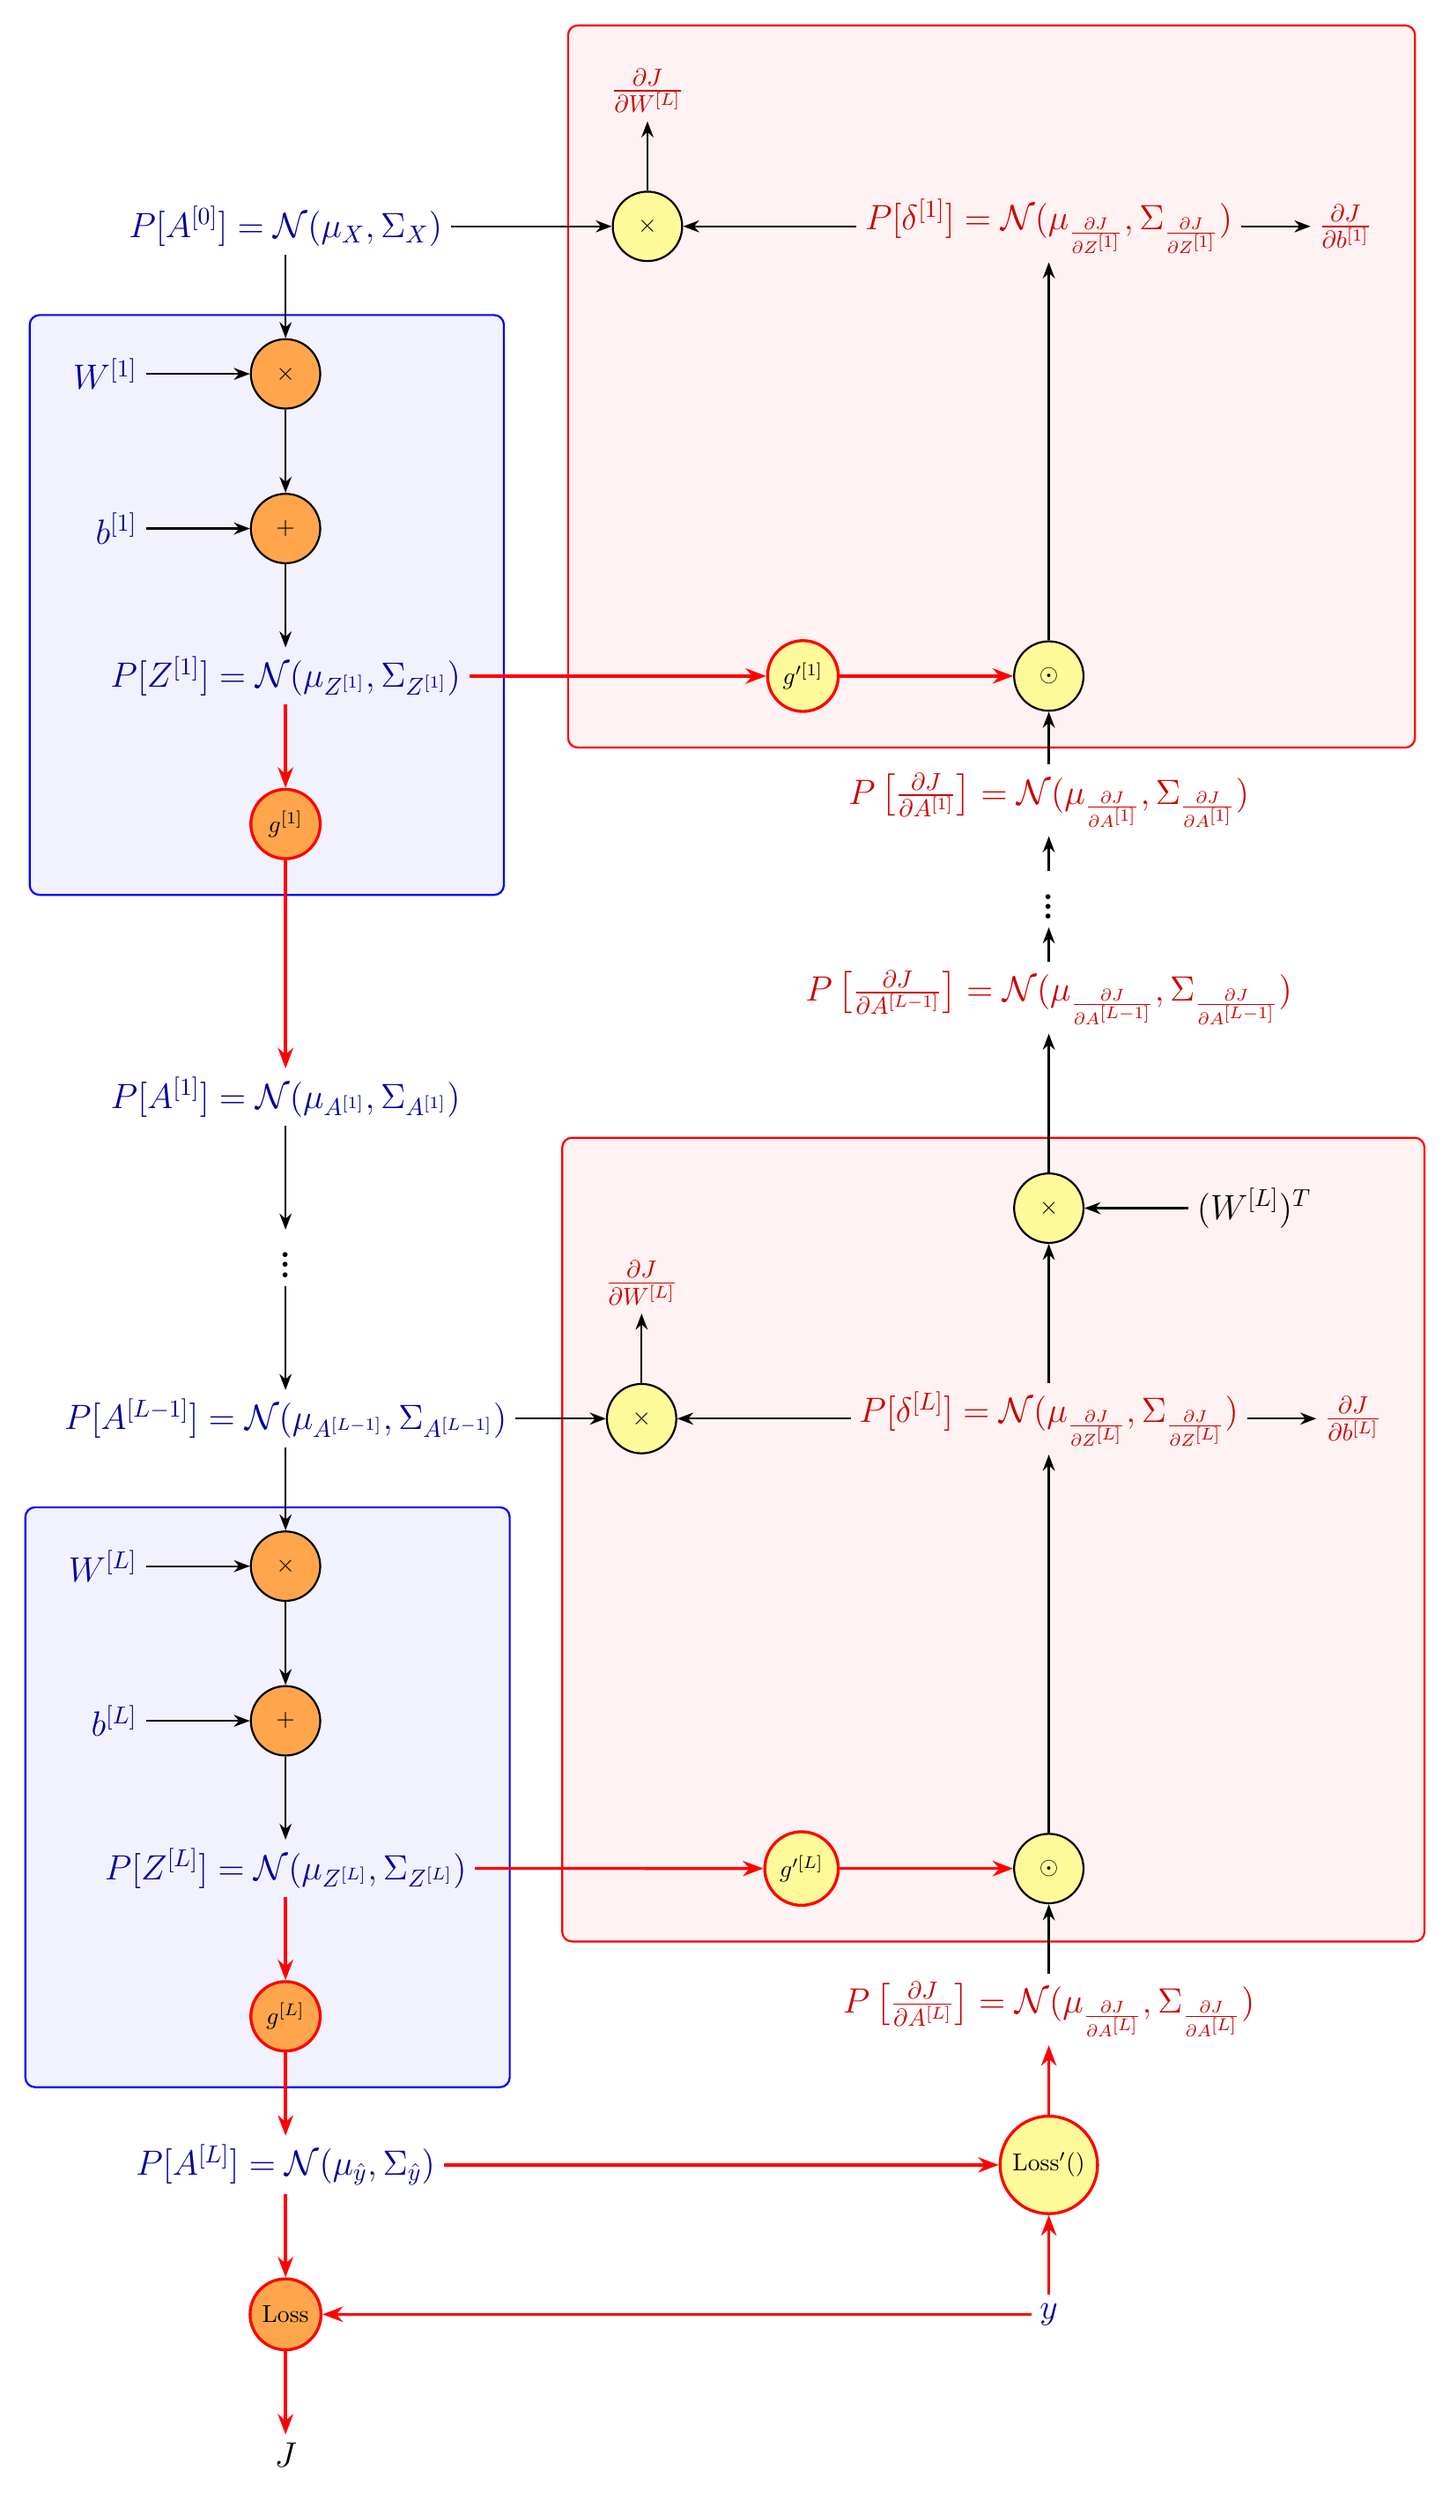
\begin{tikzpicture}[
        node distance=1.5cm and 2.5cm,
        op/.style={circle, draw, thick, minimum size=1cm, fill=yellow!40},
        fwd_op/.style={op, fill=orange!70}, % Style for forward-pass operators
        nonlinear_op/.style={draw=red, very thick}, % Style for non-linear operations
        arrow/.style={Stealth-, thick}, % Arrows flow backwards (B to A in \draw (A)--(B))
        arrow_fwd/.style={-Stealth, thick}, % Arrows for forward pass
        nonlinear_arrow_fwd/.style={arrow_fwd, red, very thick}, % Red arrows for forward non-linear
        nonlinear_arrow_back/.style={arrow, red, very thick}, % Red arrows for backward non-linear
        data/.style={font=\Large},
        grad/.style={font=\Large, text=red!80!black},
        fwd_data/.style={font=\Large, text=blue!60!black},
        layerbox/.style={draw, thick, red, rounded corners, inner sep=0.5cm, fill=red!5},
        fwd_layerbox/.style={draw, thick, blue, rounded corners, inner sep=0.5cm, fill=blue!5}
    ]
    % --- Set up layers to draw boxes in the background ---
    \pgfdeclarelayer{background}
    \pgfsetlayers{background,main}    
    
    \node[fwd_data] (A_0) {$P[A^{[0]}] = \mathcal{N}(\mu_X, \Sigma_X)$};
    \node[fwd_op, below = 1.2cm of A_0] (fwd_mult_1) {$\times$};
    \node[fwd_data, left = 1.5cm of fwd_mult_1] (W_1) {$W^{[1]}$};
    \node[fwd_op, below = 1.2cm of fwd_mult_1] (fwd_add_1) {$+$};
    \node[fwd_data, left = 1.5cm of fwd_add_1] (b_1_fwd) {$b^{[1]}$};
    \node[fwd_data, below = 1.2cm of fwd_add_1] (Z_1) {$P[Z^{[1]}] = \mathcal{N}(\mu_{Z^{[1]}}, \Sigma_{Z^{[1]}})$};

    % Connection from Z_1 to A_1
    \node[fwd_op, nonlinear_op, below = 1.2cm of Z_1] (g_1) {$g^{[1]}$};
    \node[fwd_data, below = 3cm of g_1] (A_1) {$P[A^{[1]}] = \mathcal{N}(\mu_{A^{[1]}}, \Sigma_{A^{[1]}})$};

    % Forward pass dots
    \node[font=\Huge, below = 1.5cm of A_1] (dots_fwd) {$\vdots$};  
    
    % --- Detailed Forward Pass for Layer L ---
    \node[fwd_data, below = 1.5cm of dots_fwd] (A_L_minus_1) {$P[A^{[L-1]}] = \mathcal{N}(\mu_{A^{[L-1]}}, \Sigma_{A^{[L-1]}})$};
    \node[fwd_op, below = 1.2cm of A_L_minus_1] (fwd_mult_L) {$\times$};
    \node[fwd_data, left = 1.5cm of fwd_mult_L] (W_L) {$W^{[L]}$};
    \node[fwd_op, below = 1.2cm of fwd_mult_L] (fwd_add_L) {$+$};
    \node[fwd_data, left = 1.5cm of fwd_add_L] (b_L_fwd) {$b^{[L]}$};
    \node[fwd_data, below = 1.2cm of fwd_add_L] (Z_L) {$P[Z^{[L]}] = \mathcal{N}(\mu_{Z^{[L]}}, \Sigma_{Z^{[L]}})$};
    \node[fwd_op, nonlinear_op, below = 1.2cm of Z_L] (g_L)  {$g^{[L]}$};
    \node[fwd_data, below = 1.2cm of g_L] (y_hat) {$P[A^{[L]}] = \mathcal{N}(\mu_{\hat{y}}, \Sigma_{\hat{y}})$};
    
    % --- Forward Pass Loss Calculation ---
    \node[fwd_op, nonlinear_op, below = 1.2cm of y_hat] (loss_func) {Loss};
    \node[data, below=1.2cm of loss_func] (J) {$J$};    
    
    % --- LOSS FUNCTION (AT THE BOTTOM) ----
    \node[op, nonlinear_op, right = 8cm of y_hat] (loss_prime) {Loss$'$()};    
    \node[fwd_data, at=(loss_prime.south |- loss_func.east)] (y) {$y$};

    % --- LAYER L (ABOVE LOSS) ---
    \node[grad, above = 1cm of loss_prime] (dA_L) {$P\left[\frac{\partial J}{\partial A^{[L]}}\right] = \mathcal{N}(\mu_{\frac{\partial J}{\partial A^{[L]}}}, \Sigma_{\frac{\partial J}{\partial A^{[L]}}})$};
    \node[op, above = 1cm of dA_L] (had1) {$\odot$};
    \node[op, nonlinear_op, left = 2.5cm of had1] (gprime_L_func) {$g'^{[L]}$};
    \node[grad, at=(had1.north |- A_L_minus_1.east)] (dZ_L) {$P[\delta^{[L]}] = \mathcal{N}(\mu_{\frac{\partial J}{\partial Z^{[L]}}}, \Sigma_{\frac{\partial J}{\partial Z^{[L]}}})$};

    \node[op, above = 2cm of dZ_L] (mult_a) {$\times$};
    \node[data, right = 1.5cm of mult_a] (W_L_T) {$(W^{[L]})^T$};
    \node[grad, above = 2cm of mult_a] (dA_L_minus_1) {$P\left[\frac{\partial J}{\partial A^{[L-1]}}\right] = \mathcal{N}(\mu_{\frac{\partial J}{\partial A^{[L-1]}}}, \Sigma_{\frac{\partial J}{\partial A^{[L-1]}}})$};

    \node[op, left = 2.5cm of dZ_L] (mult_w) {$\times$};
    \node[grad, above  = 1cm of mult_w] (dW_L) {$\frac{\partial J}{\partial W^{[L]}}$};
    \node[grad, right = 1cm of dZ_L] (db_L) {$\frac{\partial J}{\partial b^{[L]}}$};

    % --- CONTINUATION DOTS (ABOVE LAYER L) ---
    \node[font=\Huge, above = 0.5cm of dA_L_minus_1] (dots) {$\vdots$};

    % --- LAYER 1 (AT THE TOP) ---
    \node[grad, above = 0.5cm of dots] (dA_1) {$P\left[\frac{\partial J}{\partial A^{[1]}}\right] = \mathcal{N}(\mu_{\frac{\partial J}{\partial A^{[1]}}}, \Sigma_{\frac{\partial J}{\partial A^{[1]}}})$};
    \node[op, at=(dA_1.north |- Z_1.east)] (had_final) {$\odot$};
    \node[op, nonlinear_op, left = 2.5cm of had_final] (gprime_1_func) {$g'^{[1]}$};
    \node[grad, at=(had_final.north |- A_0.east)] (dZ_1) {$P[\delta^{[1]}] = \mathcal{N}(\mu_{\frac{\partial J}{\partial Z^{[1]}}}, \Sigma_{\frac{\partial J}{\partial Z^{[1]}}})$};

    \node[op, left = 2.5cm of dZ_1] (mult_w_final) {$\times$};
    \node[grad, above = 1cm of mult_w_final] (dW_1) {$\frac{\partial J}{\partial W^{[L]}}$};
    \node[grad, right = 1cm of dZ_1] (db_1) {$\frac{\partial J}{\partial b^{[1]}}$};

    % --- ARROWS ---
    % Forward Pass Arrows
    \draw[nonlinear_arrow_fwd] (y_hat) -- (loss_func);
    \draw[nonlinear_arrow_fwd] (y) -- (loss_func);
    \draw[nonlinear_arrow_fwd] (loss_func) -- (J);
    \draw[nonlinear_arrow_fwd] (Z_L) -- (g_L);
    \draw[nonlinear_arrow_fwd] (g_L) -- (y_hat);
    \draw[arrow_fwd] (A_L_minus_1) -- (fwd_mult_L);
    \draw[arrow_fwd] (W_L) -- (fwd_mult_L);
    \draw[arrow_fwd] (fwd_mult_L) -- (fwd_add_L);
    \draw[arrow_fwd] (b_L_fwd) -- (fwd_add_L);
    \draw[arrow_fwd] (fwd_add_L) -- (Z_L);
    \draw[arrow_fwd] (A_0) -- (fwd_mult_1);
    \draw[arrow_fwd] (W_1) -- (fwd_mult_1);
    \draw[arrow_fwd] (fwd_mult_1) -- (fwd_add_1);
    \draw[arrow_fwd] (b_1_fwd) -- (fwd_add_1);
    \draw[arrow_fwd] (fwd_add_1) -- (Z_1);
    \draw[nonlinear_arrow_fwd] (Z_1) -- (g_1);
    \draw[nonlinear_arrow_fwd] (g_1) -- (A_1);
    \draw[arrow_fwd] (A_1) -- (dots_fwd);
    \draw[arrow_fwd] (dots_fwd) -- (A_L_minus_1);

    % Backpropagation Arrows
    \draw[nonlinear_arrow_back] (loss_prime) -- (y_hat);
    \draw[nonlinear_arrow_back] (loss_prime) -- (y);
    \draw[nonlinear_arrow_back] (dA_L) -- (loss_prime);
    \draw[arrow] (had1) -- (dA_L);
    \draw[nonlinear_arrow_back] (had1) -- (gprime_L_func);
    \draw[nonlinear_arrow_back] (gprime_L_func) -- (Z_L);
    \draw[arrow] (dZ_L) -- (had1);
    \draw[arrow] (mult_w) -- (dZ_L);
    \draw[arrow] (mult_w) -- (A_L_minus_1);
    \draw[arrow] (dW_L) -- (mult_w);
    \draw[arrow] (db_L) -- (dZ_L);
    \draw[arrow] (mult_a) -- (dZ_L);
    \draw[arrow] (mult_a) -- (W_L_T);
    \draw[arrow] (dA_L_minus_1) -- (mult_a);
    \draw[arrow] (dots) -- (dA_L_minus_1);
    \draw[arrow] (dA_1) -- (dots);
    \draw[arrow] (had_final) -- (dA_1);
    \draw[nonlinear_arrow_back] (had_final) -- (gprime_1_func);
    \draw[nonlinear_arrow_back] (gprime_1_func) -- (Z_1);
    \draw[arrow] (dZ_1) -- (had_final);
    \draw[arrow] (mult_w_final) -- (dZ_1);
    \draw[arrow] (mult_w_final) -- (A_0);
    \draw[arrow] (dW_1) -- (mult_w_final);
    \draw[arrow] (db_1) -- (dZ_1);

\begin{pgfonlayer}{background}
    % Box for Layer L (Backpropagation)
    \node[layerbox,
          fit=(gprime_L_func) (had1) (dZ_L) (mult_a) (W_L_T) (dW_L) (db_L) ] {};
    % Box for Layer 1 (Backpropagation)
    \node[layerbox,
          fit=(gprime_1_func) (had_final) (dZ_1) (mult_w_final) (dW_1) (db_1)] {};
    % New box for Layer L (Forward Pass)
    \node[fwd_layerbox,
          fit=(W_L) (Z_L) (g_L)] {};
    % New box for Layer 1 (Forward Pass)
    \node[fwd_layerbox,
          fit=(W_1) (Z_1) (g_1)] {};
\end{pgfonlayer}

    \end{tikzpicture}%
}

\ifdefined\ispartofbook
  % This part is intentionally left blank when included in the main book.
  % The \newcommand is defined, and the chapter file is responsible for calling it.
\else
  % This part is for standalone compilation of the image.
  \combineddiagram 
  \end{document}
\fi
